% Created by tikzDevice version 0.10.1 on 2018-01-16 22:08:40
% !TEX encoding = UTF-8 Unicode
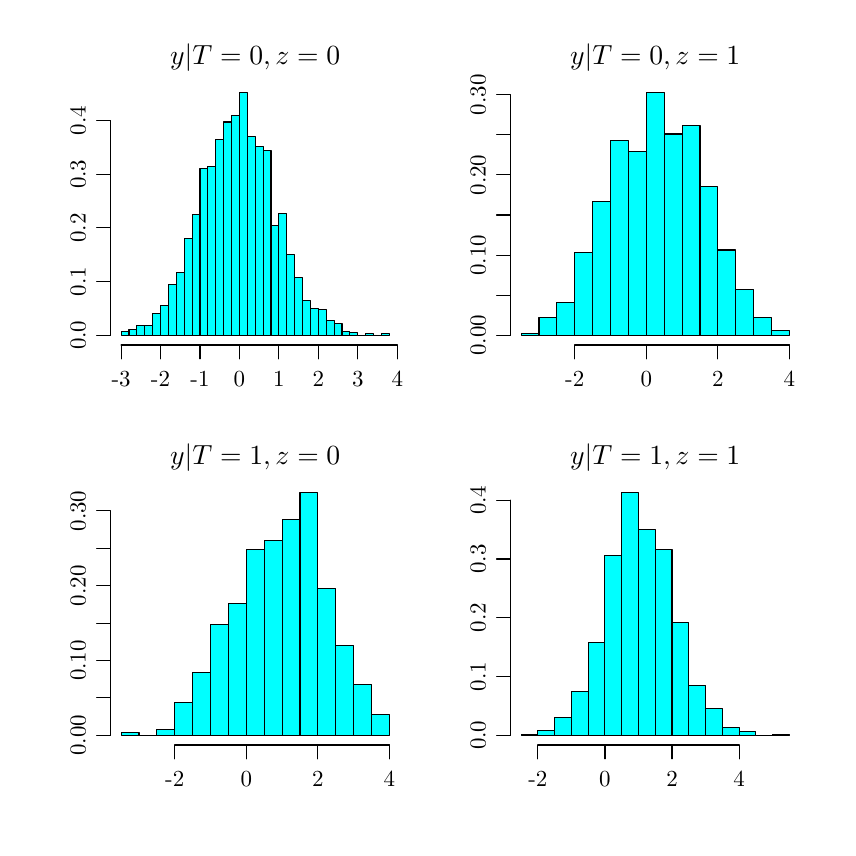
\begin{tikzpicture}[x=1pt,y=1pt]
\definecolor{fillColor}{RGB}{255,255,255}
\path[use as bounding box,fill=fillColor,fill opacity=0.00] (0,0) rectangle (289.08,289.08);
\begin{scope}
\path[clip] (  0.00,  0.00) rectangle (289.08,289.08);
\definecolor{drawColor}{RGB}{0,0,0}

\path[draw=drawColor,line width= 0.4pt,line join=round,line cap=round] ( 33.76,174.42) -- (133.56,174.42);

\path[draw=drawColor,line width= 0.4pt,line join=round,line cap=round] ( 33.76,174.42) -- ( 33.76,169.44);

\path[draw=drawColor,line width= 0.4pt,line join=round,line cap=round] ( 48.02,174.42) -- ( 48.02,169.44);

\path[draw=drawColor,line width= 0.4pt,line join=round,line cap=round] ( 62.27,174.42) -- ( 62.27,169.44);

\path[draw=drawColor,line width= 0.4pt,line join=round,line cap=round] ( 76.53,174.42) -- ( 76.53,169.44);

\path[draw=drawColor,line width= 0.4pt,line join=round,line cap=round] ( 90.79,174.42) -- ( 90.79,169.44);

\path[draw=drawColor,line width= 0.4pt,line join=round,line cap=round] (105.04,174.42) -- (105.04,169.44);

\path[draw=drawColor,line width= 0.4pt,line join=round,line cap=round] (119.30,174.42) -- (119.30,169.44);

\path[draw=drawColor,line width= 0.4pt,line join=round,line cap=round] (133.56,174.42) -- (133.56,169.44);

\node[text=drawColor,anchor=base,inner sep=0pt, outer sep=0pt, scale=  0.83] at ( 33.76,159.48) {-3};

\node[text=drawColor,anchor=base,inner sep=0pt, outer sep=0pt, scale=  0.83] at ( 48.02,159.48) {-2};

\node[text=drawColor,anchor=base,inner sep=0pt, outer sep=0pt, scale=  0.83] at ( 62.27,159.48) {-1};

\node[text=drawColor,anchor=base,inner sep=0pt, outer sep=0pt, scale=  0.83] at ( 76.53,159.48) {0};

\node[text=drawColor,anchor=base,inner sep=0pt, outer sep=0pt, scale=  0.83] at ( 90.79,159.48) {1};

\node[text=drawColor,anchor=base,inner sep=0pt, outer sep=0pt, scale=  0.83] at (105.04,159.48) {2};

\node[text=drawColor,anchor=base,inner sep=0pt, outer sep=0pt, scale=  0.83] at (119.30,159.48) {3};

\node[text=drawColor,anchor=base,inner sep=0pt, outer sep=0pt, scale=  0.83] at (133.56,159.48) {4};

\path[draw=drawColor,line width= 0.4pt,line join=round,line cap=round] ( 29.88,177.93) -- ( 29.88,255.51);

\path[draw=drawColor,line width= 0.4pt,line join=round,line cap=round] ( 29.88,177.93) -- ( 24.90,177.93);

\path[draw=drawColor,line width= 0.4pt,line join=round,line cap=round] ( 29.88,197.32) -- ( 24.90,197.32);

\path[draw=drawColor,line width= 0.4pt,line join=round,line cap=round] ( 29.88,216.72) -- ( 24.90,216.72);

\path[draw=drawColor,line width= 0.4pt,line join=round,line cap=round] ( 29.88,236.12) -- ( 24.90,236.12);

\path[draw=drawColor,line width= 0.4pt,line join=round,line cap=round] ( 29.88,255.51) -- ( 24.90,255.51);

\node[text=drawColor,rotate= 90.00,anchor=base,inner sep=0pt, outer sep=0pt, scale=  0.83] at ( 20.92,177.93) {0.0};

\node[text=drawColor,rotate= 90.00,anchor=base,inner sep=0pt, outer sep=0pt, scale=  0.83] at ( 20.92,197.32) {0.1};

\node[text=drawColor,rotate= 90.00,anchor=base,inner sep=0pt, outer sep=0pt, scale=  0.83] at ( 20.92,216.72) {0.2};

\node[text=drawColor,rotate= 90.00,anchor=base,inner sep=0pt, outer sep=0pt, scale=  0.83] at ( 20.92,236.12) {0.3};

\node[text=drawColor,rotate= 90.00,anchor=base,inner sep=0pt, outer sep=0pt, scale=  0.83] at ( 20.92,255.51) {0.4};
\end{scope}
\begin{scope}
\path[clip] (  0.00,144.54) rectangle (144.54,289.08);
\definecolor{drawColor}{RGB}{0,0,0}

\node[text=drawColor,anchor=base,inner sep=0pt, outer sep=0pt, scale=  1.00] at ( 82.23,275.68) {\bfseries $y|T=0,z=0$};
\end{scope}
\begin{scope}
\path[clip] ( 29.88,174.42) rectangle (134.58,269.16);
\definecolor{drawColor}{RGB}{0,0,0}
\definecolor{fillColor}{RGB}{0,255,255}

\path[draw=drawColor,line width= 0.4pt,line join=round,line cap=round,fill=fillColor] ( 33.76,177.93) rectangle ( 36.61,179.38);

\path[draw=drawColor,line width= 0.4pt,line join=round,line cap=round,fill=fillColor] ( 36.61,177.93) rectangle ( 39.46,179.87);

\path[draw=drawColor,line width= 0.4pt,line join=round,line cap=round,fill=fillColor] ( 39.46,177.93) rectangle ( 42.31,181.32);

\path[draw=drawColor,line width= 0.4pt,line join=round,line cap=round,fill=fillColor] ( 42.31,177.93) rectangle ( 45.16,181.32);

\path[draw=drawColor,line width= 0.4pt,line join=round,line cap=round,fill=fillColor] ( 45.16,177.93) rectangle ( 48.01,185.68);

\path[draw=drawColor,line width= 0.4pt,line join=round,line cap=round,fill=fillColor] ( 48.01,177.93) rectangle ( 50.87,188.59);

\path[draw=drawColor,line width= 0.4pt,line join=round,line cap=round,fill=fillColor] ( 50.87,177.93) rectangle ( 53.72,196.35);

\path[draw=drawColor,line width= 0.4pt,line join=round,line cap=round,fill=fillColor] ( 53.72,177.93) rectangle ( 56.57,200.71);

\path[draw=drawColor,line width= 0.4pt,line join=round,line cap=round,fill=fillColor] ( 56.57,177.93) rectangle ( 59.42,212.82);

\path[draw=drawColor,line width= 0.4pt,line join=round,line cap=round,fill=fillColor] ( 59.42,177.93) rectangle ( 62.27,221.55);

\path[draw=drawColor,line width= 0.4pt,line join=round,line cap=round,fill=fillColor] ( 62.27,177.93) rectangle ( 65.12,238.03);

\path[draw=drawColor,line width= 0.4pt,line join=round,line cap=round,fill=fillColor] ( 65.12,177.93) rectangle ( 67.97,239.00);

\path[draw=drawColor,line width= 0.4pt,line join=round,line cap=round,fill=fillColor] ( 67.97,177.93) rectangle ( 70.82,248.69);

\path[draw=drawColor,line width= 0.4pt,line join=round,line cap=round,fill=fillColor] ( 70.82,177.93) rectangle ( 73.68,254.99);

\path[draw=drawColor,line width= 0.4pt,line join=round,line cap=round,fill=fillColor] ( 73.68,177.93) rectangle ( 76.53,257.41);

\path[draw=drawColor,line width= 0.4pt,line join=round,line cap=round,fill=fillColor] ( 76.53,177.93) rectangle ( 79.38,265.65);

\path[draw=drawColor,line width= 0.4pt,line join=round,line cap=round,fill=fillColor] ( 79.38,177.93) rectangle ( 82.23,249.66);

\path[draw=drawColor,line width= 0.4pt,line join=round,line cap=round,fill=fillColor] ( 82.23,177.93) rectangle ( 85.08,246.26);

\path[draw=drawColor,line width= 0.4pt,line join=round,line cap=round,fill=fillColor] ( 85.08,177.93) rectangle ( 87.93,244.81);

\path[draw=drawColor,line width= 0.4pt,line join=round,line cap=round,fill=fillColor] ( 87.93,177.93) rectangle ( 90.78,217.67);

\path[draw=drawColor,line width= 0.4pt,line join=round,line cap=round,fill=fillColor] ( 90.78,177.93) rectangle ( 93.64,222.03);

\path[draw=drawColor,line width= 0.4pt,line join=round,line cap=round,fill=fillColor] ( 93.64,177.93) rectangle ( 96.49,207.01);

\path[draw=drawColor,line width= 0.4pt,line join=round,line cap=round,fill=fillColor] ( 96.49,177.93) rectangle ( 99.34,198.77);

\path[draw=drawColor,line width= 0.4pt,line join=round,line cap=round,fill=fillColor] ( 99.34,177.93) rectangle (102.19,190.53);

\path[draw=drawColor,line width= 0.4pt,line join=round,line cap=round,fill=fillColor] (102.19,177.93) rectangle (105.04,187.62);

\path[draw=drawColor,line width= 0.4pt,line join=round,line cap=round,fill=fillColor] (105.04,177.93) rectangle (107.89,187.14);

\path[draw=drawColor,line width= 0.4pt,line join=round,line cap=round,fill=fillColor] (107.89,177.93) rectangle (110.74,183.26);

\path[draw=drawColor,line width= 0.4pt,line join=round,line cap=round,fill=fillColor] (110.74,177.93) rectangle (113.59,182.29);

\path[draw=drawColor,line width= 0.4pt,line join=round,line cap=round,fill=fillColor] (113.59,177.93) rectangle (116.45,179.38);

\path[draw=drawColor,line width= 0.4pt,line join=round,line cap=round,fill=fillColor] (116.45,177.93) rectangle (119.30,178.90);

\path[draw=drawColor,line width= 0.4pt,line join=round,line cap=round,fill=fillColor] (119.30,177.93) rectangle (122.15,177.93);

\path[draw=drawColor,line width= 0.4pt,line join=round,line cap=round,fill=fillColor] (122.15,177.93) rectangle (125.00,178.41);

\path[draw=drawColor,line width= 0.4pt,line join=round,line cap=round,fill=fillColor] (125.00,177.93) rectangle (127.85,177.93);

\path[draw=drawColor,line width= 0.4pt,line join=round,line cap=round,fill=fillColor] (127.85,177.93) rectangle (130.70,178.41);
\end{scope}
\begin{scope}
\path[clip] (  0.00,  0.00) rectangle (289.08,289.08);
\definecolor{drawColor}{RGB}{0,0,0}

\path[draw=drawColor,line width= 0.4pt,line join=round,line cap=round] (197.69,174.42) -- (275.25,174.42);

\path[draw=drawColor,line width= 0.4pt,line join=round,line cap=round] (197.69,174.42) -- (197.69,169.44);

\path[draw=drawColor,line width= 0.4pt,line join=round,line cap=round] (223.54,174.42) -- (223.54,169.44);

\path[draw=drawColor,line width= 0.4pt,line join=round,line cap=round] (249.40,174.42) -- (249.40,169.44);

\path[draw=drawColor,line width= 0.4pt,line join=round,line cap=round] (275.25,174.42) -- (275.25,169.44);

\node[text=drawColor,anchor=base,inner sep=0pt, outer sep=0pt, scale=  0.83] at (197.69,159.48) {-2};

\node[text=drawColor,anchor=base,inner sep=0pt, outer sep=0pt, scale=  0.83] at (223.54,159.48) {0};

\node[text=drawColor,anchor=base,inner sep=0pt, outer sep=0pt, scale=  0.83] at (249.40,159.48) {2};

\node[text=drawColor,anchor=base,inner sep=0pt, outer sep=0pt, scale=  0.83] at (275.25,159.48) {4};

\path[draw=drawColor,line width= 0.4pt,line join=round,line cap=round] (174.42,177.93) -- (174.42,264.82);

\path[draw=drawColor,line width= 0.4pt,line join=round,line cap=round] (174.42,177.93) -- (169.44,177.93);

\path[draw=drawColor,line width= 0.4pt,line join=round,line cap=round] (174.42,192.41) -- (169.44,192.41);

\path[draw=drawColor,line width= 0.4pt,line join=round,line cap=round] (174.42,206.89) -- (169.44,206.89);

\path[draw=drawColor,line width= 0.4pt,line join=round,line cap=round] (174.42,221.38) -- (169.44,221.38);

\path[draw=drawColor,line width= 0.4pt,line join=round,line cap=round] (174.42,235.86) -- (169.44,235.86);

\path[draw=drawColor,line width= 0.4pt,line join=round,line cap=round] (174.42,250.34) -- (169.44,250.34);

\path[draw=drawColor,line width= 0.4pt,line join=round,line cap=round] (174.42,264.82) -- (169.44,264.82);

\node[text=drawColor,rotate= 90.00,anchor=base,inner sep=0pt, outer sep=0pt, scale=  0.83] at (165.46,177.93) {0.00};

\node[text=drawColor,rotate= 90.00,anchor=base,inner sep=0pt, outer sep=0pt, scale=  0.83] at (165.46,206.89) {0.10};

\node[text=drawColor,rotate= 90.00,anchor=base,inner sep=0pt, outer sep=0pt, scale=  0.83] at (165.46,235.86) {0.20};

\node[text=drawColor,rotate= 90.00,anchor=base,inner sep=0pt, outer sep=0pt, scale=  0.83] at (165.46,264.82) {0.30};
\end{scope}
\begin{scope}
\path[clip] (144.54,144.54) rectangle (289.08,289.08);
\definecolor{drawColor}{RGB}{0,0,0}

\node[text=drawColor,anchor=base,inner sep=0pt, outer sep=0pt, scale=  1.00] at (226.77,275.68) {\bfseries $y|T=0,z=1$};
\end{scope}
\begin{scope}
\path[clip] (174.42,174.42) rectangle (279.12,269.16);
\definecolor{drawColor}{RGB}{0,0,0}
\definecolor{fillColor}{RGB}{0,255,255}

\path[draw=drawColor,line width= 0.4pt,line join=round,line cap=round,fill=fillColor] (178.30,177.93) rectangle (184.76,178.72);

\path[draw=drawColor,line width= 0.4pt,line join=round,line cap=round,fill=fillColor] (184.76,177.93) rectangle (191.22,184.25);

\path[draw=drawColor,line width= 0.4pt,line join=round,line cap=round,fill=fillColor] (191.22,177.93) rectangle (197.69,189.78);

\path[draw=drawColor,line width= 0.4pt,line join=round,line cap=round,fill=fillColor] (197.69,177.93) rectangle (204.15,207.96);

\path[draw=drawColor,line width= 0.4pt,line join=round,line cap=round,fill=fillColor] (204.15,177.93) rectangle (210.61,226.14);

\path[draw=drawColor,line width= 0.4pt,line join=round,line cap=round,fill=fillColor] (210.61,177.93) rectangle (217.08,248.26);

\path[draw=drawColor,line width= 0.4pt,line join=round,line cap=round,fill=fillColor] (217.08,177.93) rectangle (223.54,244.31);

\path[draw=drawColor,line width= 0.4pt,line join=round,line cap=round,fill=fillColor] (223.54,177.93) rectangle (230.00,265.65);

\path[draw=drawColor,line width= 0.4pt,line join=round,line cap=round,fill=fillColor] (230.00,177.93) rectangle (236.46,250.64);

\path[draw=drawColor,line width= 0.4pt,line join=round,line cap=round,fill=fillColor] (236.46,177.93) rectangle (242.93,253.80);

\path[draw=drawColor,line width= 0.4pt,line join=round,line cap=round,fill=fillColor] (242.93,177.93) rectangle (249.39,231.67);

\path[draw=drawColor,line width= 0.4pt,line join=round,line cap=round,fill=fillColor] (249.39,177.93) rectangle (255.85,208.75);

\path[draw=drawColor,line width= 0.4pt,line join=round,line cap=round,fill=fillColor] (255.85,177.93) rectangle (262.32,194.52);

\path[draw=drawColor,line width= 0.4pt,line join=round,line cap=round,fill=fillColor] (262.32,177.93) rectangle (268.78,184.25);

\path[draw=drawColor,line width= 0.4pt,line join=round,line cap=round,fill=fillColor] (268.78,177.93) rectangle (275.24,179.51);
\end{scope}
\begin{scope}
\path[clip] (  0.00,  0.00) rectangle (289.08,289.08);
\definecolor{drawColor}{RGB}{0,0,0}

\path[draw=drawColor,line width= 0.4pt,line join=round,line cap=round] ( 53.15, 29.88) -- (130.71, 29.88);

\path[draw=drawColor,line width= 0.4pt,line join=round,line cap=round] ( 53.15, 29.88) -- ( 53.15, 24.90);

\path[draw=drawColor,line width= 0.4pt,line join=round,line cap=round] ( 79.00, 29.88) -- ( 79.00, 24.90);

\path[draw=drawColor,line width= 0.4pt,line join=round,line cap=round] (104.86, 29.88) -- (104.86, 24.90);

\path[draw=drawColor,line width= 0.4pt,line join=round,line cap=round] (130.71, 29.88) -- (130.71, 24.90);

\node[text=drawColor,anchor=base,inner sep=0pt, outer sep=0pt, scale=  0.83] at ( 53.15, 14.94) {-2};

\node[text=drawColor,anchor=base,inner sep=0pt, outer sep=0pt, scale=  0.83] at ( 79.00, 14.94) {0};

\node[text=drawColor,anchor=base,inner sep=0pt, outer sep=0pt, scale=  0.83] at (104.86, 14.94) {2};

\node[text=drawColor,anchor=base,inner sep=0pt, outer sep=0pt, scale=  0.83] at (130.71, 14.94) {4};

\path[draw=drawColor,line width= 0.4pt,line join=round,line cap=round] ( 29.88, 33.39) -- ( 29.88,114.45);

\path[draw=drawColor,line width= 0.4pt,line join=round,line cap=round] ( 29.88, 33.39) -- ( 24.90, 33.39);

\path[draw=drawColor,line width= 0.4pt,line join=round,line cap=round] ( 29.88, 46.90) -- ( 24.90, 46.90);

\path[draw=drawColor,line width= 0.4pt,line join=round,line cap=round] ( 29.88, 60.41) -- ( 24.90, 60.41);

\path[draw=drawColor,line width= 0.4pt,line join=round,line cap=round] ( 29.88, 73.92) -- ( 24.90, 73.92);

\path[draw=drawColor,line width= 0.4pt,line join=round,line cap=round] ( 29.88, 87.43) -- ( 24.90, 87.43);

\path[draw=drawColor,line width= 0.4pt,line join=round,line cap=round] ( 29.88,100.94) -- ( 24.90,100.94);

\path[draw=drawColor,line width= 0.4pt,line join=round,line cap=round] ( 29.88,114.45) -- ( 24.90,114.45);

\node[text=drawColor,rotate= 90.00,anchor=base,inner sep=0pt, outer sep=0pt, scale=  0.83] at ( 20.92, 33.39) {0.00};

\node[text=drawColor,rotate= 90.00,anchor=base,inner sep=0pt, outer sep=0pt, scale=  0.83] at ( 20.92, 60.41) {0.10};

\node[text=drawColor,rotate= 90.00,anchor=base,inner sep=0pt, outer sep=0pt, scale=  0.83] at ( 20.92, 87.43) {0.20};

\node[text=drawColor,rotate= 90.00,anchor=base,inner sep=0pt, outer sep=0pt, scale=  0.83] at ( 20.92,114.45) {0.30};
\end{scope}
\begin{scope}
\path[clip] (  0.00,  0.00) rectangle (144.54,144.54);
\definecolor{drawColor}{RGB}{0,0,0}

\node[text=drawColor,anchor=base,inner sep=0pt, outer sep=0pt, scale=  1.00] at ( 82.23,131.14) {\bfseries $y|T=1,z=0$};
\end{scope}
\begin{scope}
\path[clip] ( 29.88, 29.88) rectangle (134.58,124.62);
\definecolor{drawColor}{RGB}{0,0,0}
\definecolor{fillColor}{RGB}{0,255,255}

\path[draw=drawColor,line width= 0.4pt,line join=round,line cap=round,fill=fillColor] ( 33.76, 33.39) rectangle ( 40.22, 34.47);

\path[draw=drawColor,line width= 0.4pt,line join=round,line cap=round,fill=fillColor] ( 40.22, 33.39) rectangle ( 46.68, 33.39);

\path[draw=drawColor,line width= 0.4pt,line join=round,line cap=round,fill=fillColor] ( 46.68, 33.39) rectangle ( 53.15, 35.55);

\path[draw=drawColor,line width= 0.4pt,line join=round,line cap=round,fill=fillColor] ( 53.15, 33.39) rectangle ( 59.61, 45.30);

\path[draw=drawColor,line width= 0.4pt,line join=round,line cap=round,fill=fillColor] ( 59.61, 33.39) rectangle ( 66.07, 56.13);

\path[draw=drawColor,line width= 0.4pt,line join=round,line cap=round,fill=fillColor] ( 66.07, 33.39) rectangle ( 72.54, 73.46);

\path[draw=drawColor,line width= 0.4pt,line join=round,line cap=round,fill=fillColor] ( 72.54, 33.39) rectangle ( 79.00, 81.04);

\path[draw=drawColor,line width= 0.4pt,line join=round,line cap=round,fill=fillColor] ( 79.00, 33.39) rectangle ( 85.46,100.53);

\path[draw=drawColor,line width= 0.4pt,line join=round,line cap=round,fill=fillColor] ( 85.46, 33.39) rectangle ( 91.92,103.78);

\path[draw=drawColor,line width= 0.4pt,line join=round,line cap=round,fill=fillColor] ( 91.92, 33.39) rectangle ( 98.39,111.36);

\path[draw=drawColor,line width= 0.4pt,line join=round,line cap=round,fill=fillColor] ( 98.39, 33.39) rectangle (104.85,121.11);

\path[draw=drawColor,line width= 0.4pt,line join=round,line cap=round,fill=fillColor] (104.85, 33.39) rectangle (111.31, 86.46);

\path[draw=drawColor,line width= 0.4pt,line join=round,line cap=round,fill=fillColor] (111.31, 33.39) rectangle (117.78, 65.88);

\path[draw=drawColor,line width= 0.4pt,line join=round,line cap=round,fill=fillColor] (117.78, 33.39) rectangle (124.24, 51.80);

\path[draw=drawColor,line width= 0.4pt,line join=round,line cap=round,fill=fillColor] (124.24, 33.39) rectangle (130.70, 40.97);
\end{scope}
\begin{scope}
\path[clip] (  0.00,  0.00) rectangle (289.08,289.08);
\definecolor{drawColor}{RGB}{0,0,0}

\path[draw=drawColor,line width= 0.4pt,line join=round,line cap=round] (184.36, 29.88) -- (257.07, 29.88);

\path[draw=drawColor,line width= 0.4pt,line join=round,line cap=round] (184.36, 29.88) -- (184.36, 24.90);

\path[draw=drawColor,line width= 0.4pt,line join=round,line cap=round] (208.60, 29.88) -- (208.60, 24.90);

\path[draw=drawColor,line width= 0.4pt,line join=round,line cap=round] (232.84, 29.88) -- (232.84, 24.90);

\path[draw=drawColor,line width= 0.4pt,line join=round,line cap=round] (257.07, 29.88) -- (257.07, 24.90);

\node[text=drawColor,anchor=base,inner sep=0pt, outer sep=0pt, scale=  0.83] at (184.36, 14.94) {-2};

\node[text=drawColor,anchor=base,inner sep=0pt, outer sep=0pt, scale=  0.83] at (208.60, 14.94) {0};

\node[text=drawColor,anchor=base,inner sep=0pt, outer sep=0pt, scale=  0.83] at (232.84, 14.94) {2};

\node[text=drawColor,anchor=base,inner sep=0pt, outer sep=0pt, scale=  0.83] at (257.07, 14.94) {4};

\path[draw=drawColor,line width= 0.4pt,line join=round,line cap=round] (174.42, 33.39) -- (174.42,118.32);

\path[draw=drawColor,line width= 0.4pt,line join=round,line cap=round] (174.42, 33.39) -- (169.44, 33.39);

\path[draw=drawColor,line width= 0.4pt,line join=round,line cap=round] (174.42, 54.62) -- (169.44, 54.62);

\path[draw=drawColor,line width= 0.4pt,line join=round,line cap=round] (174.42, 75.86) -- (169.44, 75.86);

\path[draw=drawColor,line width= 0.4pt,line join=round,line cap=round] (174.42, 97.09) -- (169.44, 97.09);

\path[draw=drawColor,line width= 0.4pt,line join=round,line cap=round] (174.42,118.32) -- (169.44,118.32);

\node[text=drawColor,rotate= 90.00,anchor=base,inner sep=0pt, outer sep=0pt, scale=  0.83] at (165.46, 33.39) {0.0};

\node[text=drawColor,rotate= 90.00,anchor=base,inner sep=0pt, outer sep=0pt, scale=  0.83] at (165.46, 54.62) {0.1};

\node[text=drawColor,rotate= 90.00,anchor=base,inner sep=0pt, outer sep=0pt, scale=  0.83] at (165.46, 75.86) {0.2};

\node[text=drawColor,rotate= 90.00,anchor=base,inner sep=0pt, outer sep=0pt, scale=  0.83] at (165.46, 97.09) {0.3};

\node[text=drawColor,rotate= 90.00,anchor=base,inner sep=0pt, outer sep=0pt, scale=  0.83] at (165.46,118.32) {0.4};
\end{scope}
\begin{scope}
\path[clip] (144.54,  0.00) rectangle (289.08,144.54);
\definecolor{drawColor}{RGB}{0,0,0}

\node[text=drawColor,anchor=base,inner sep=0pt, outer sep=0pt, scale=  1.00] at (226.77,131.14) {\bfseries $y|T=1,z=1$};
\end{scope}
\begin{scope}
\path[clip] (174.42, 29.88) rectangle (279.12,124.62);
\definecolor{drawColor}{RGB}{0,0,0}
\definecolor{fillColor}{RGB}{0,255,255}

\path[draw=drawColor,line width= 0.4pt,line join=round,line cap=round,fill=fillColor] (178.30, 33.39) rectangle (184.36, 33.63);

\path[draw=drawColor,line width= 0.4pt,line join=round,line cap=round,fill=fillColor] (184.36, 33.39) rectangle (190.42, 35.07);

\path[draw=drawColor,line width= 0.4pt,line join=round,line cap=round,fill=fillColor] (190.42, 33.39) rectangle (196.47, 39.88);

\path[draw=drawColor,line width= 0.4pt,line join=round,line cap=round,fill=fillColor] (196.47, 33.39) rectangle (202.53, 49.25);

\path[draw=drawColor,line width= 0.4pt,line join=round,line cap=round,fill=fillColor] (202.53, 33.39) rectangle (208.59, 66.80);

\path[draw=drawColor,line width= 0.4pt,line join=round,line cap=round,fill=fillColor] (208.59, 33.39) rectangle (214.65, 98.28);

\path[draw=drawColor,line width= 0.4pt,line join=round,line cap=round,fill=fillColor] (214.65, 33.39) rectangle (220.71,121.11);

\path[draw=drawColor,line width= 0.4pt,line join=round,line cap=round,fill=fillColor] (220.71, 33.39) rectangle (226.77,107.65);

\path[draw=drawColor,line width= 0.4pt,line join=round,line cap=round,fill=fillColor] (226.77, 33.39) rectangle (232.83,100.44);

\path[draw=drawColor,line width= 0.4pt,line join=round,line cap=round,fill=fillColor] (232.83, 33.39) rectangle (238.89, 74.25);

\path[draw=drawColor,line width= 0.4pt,line join=round,line cap=round,fill=fillColor] (238.89, 33.39) rectangle (244.95, 51.41);

\path[draw=drawColor,line width= 0.4pt,line join=round,line cap=round,fill=fillColor] (244.95, 33.39) rectangle (251.01, 43.00);

\path[draw=drawColor,line width= 0.4pt,line join=round,line cap=round,fill=fillColor] (251.01, 33.39) rectangle (257.07, 36.27);

\path[draw=drawColor,line width= 0.4pt,line join=round,line cap=round,fill=fillColor] (257.07, 33.39) rectangle (263.12, 34.83);

\path[draw=drawColor,line width= 0.4pt,line join=round,line cap=round,fill=fillColor] (263.12, 33.39) rectangle (269.18, 33.39);

\path[draw=drawColor,line width= 0.4pt,line join=round,line cap=round,fill=fillColor] (269.18, 33.39) rectangle (275.24, 33.63);
\end{scope}
\end{tikzpicture}
